\documentclass[11pt,a4paper]{article}
\usepackage[margin=2.5cm]{geometry}
\usepackage{amsmath,amssymb}
\usepackage{booktabs}
\usepackage{siunitx}
\usepackage{graphicx}
\usepackage{pgfplots}
\pgfplotsset{compat=1.17}
\usepackage[hidelinks]{hyperref}
\usepackage{caption}
\captionsetup{font=small,labelfont=bf}
\usepackage{microtype}
\usepackage{natbib}

\title{\textbf{Wave-Tank Calibration and Validation of an Accelerometer-Based
Drifting Wave Buoy}\\[4pt]
\large Height response, period response, and operating-envelope characterization
of the Sargassum drifter wave-sensing module}
\author{Nebli / Hover --- Sargassum Drifter Program\\
\small Bench instrumentation and remote test conduct: engineering (remote); tank operation: field team (Miami)}
\date{16 July 2026}

\begin{document}
\maketitle

\begin{abstract}
\noindent
A low-cost drifting wave buoy --- a sealed sensor bottle built around a
6-axis MEMS IMU sampling vertical acceleration at \SI{10}{\hertz}, with
on-board spectral processing on an ESP32-S3 --- was calibrated and validated
in a \SI{10}{\meter} laboratory wave flume under monochromatic paddle-generated
waves. Ground-truth wave heights were obtained by frame-by-frame video analysis
of a wall-mounted ruler at the buoy's station. Across six wave heights
($H = \SIrange{10}{48}{\milli\meter}$ at \SI{0.5}{\hertz}), the on-board
significant-wave-height estimate followed the affine relation
$H_s = 1.689\,H - 8.48$~mm ($R^2 = 0.9995$, RMSE \SI{0.45}{\milli\meter}),
and the inverse map transferred to an independent \SI{0.4}{\hertz} validation
point within the ground-truth measurement band. The peak-period estimate was
exact to within instrument resolution at all five achievable tank frequencies
(\SIrange{0.2}{1.5}{\hertz}; periods \SIrange{0.7}{5.0}{\second}), with peak-frequency
errors $\le 2\%$. Secondary findings include direct spectral identification of
the flume's fundamental seiche at \SI{0.097}{\hertz} (Merian prediction
\SI{0.099}{\hertz} at \SI{0.4}{\meter} depth), quantification of harmonic
content under large paddle strokes (20\% of in-band acceleration energy at the
first harmonic), an indication of buoy heave resonance near \SI{1}{\hertz},
and practical limits of the facility above \SI{1.5}{\hertz}. The results
support field deployment of the module for swell-band period reporting, with
height reporting subject to the fitted affine calibration and a per-frequency
response correction to be refined in future mixed-sea (wind) testing.
\end{abstract}

\section{Introduction and objectives}
The Sargassum drifter is a low-cost expendable surface buoy whose wave-sensing
module reports bulk wave parameters --- significant wave height ($H_s$) and
peak period ($T_p$) --- over a wireless telemetry link. Before ocean
deployment, the module required (i)~an absolute height calibration against
independently measured waves, (ii)~validation of the period estimate across
the frequency band of interest, and (iii)~characterization of the operating
envelope (detection floor, filter-band placement, mooring/tether effects,
platform response).

The specific objectives of this test campaign were:
\begin{enumerate}
  \item Determine the transfer between true crest-to-trough wave height $H$
        at the buoy and the on-board estimate $H_s$, at fixed frequency.
  \item Validate the on-board $T_p$ estimate against the wavemaker drive
        frequency across the achievable range.
  \item Verify the height calibration at an independent frequency and
        amplitude (transfer check).
  \item Identify facility and platform artifacts (basin seiche, wave
        harmonics, tether loading, drift) that bear on data interpretation.
\end{enumerate}

\section{Instrument}
\label{sec:instrument}
The buoy is a sealed cylindrical bottle (nominal displacement
$\sim$\SI{1}{\liter} class) containing:

\begin{itemize}
  \item \textbf{Sensing.} A QMI8658 6-axis MEMS IMU (accelerometer range
        $\pm 4g$, internal ODR \SI{1}{\kilo\hertz}). Vertical (heave)
        acceleration is derived from attitude-corrected specific force with
        gravity removed, decimated to \SI{10}{\hertz}.
  \item \textbf{On-board processing.} A sliding window of $N = 1024$ heave
        samples (\SI{102.4}{\second} at \SI{10}{\hertz}) is transformed
        (FFT); a configurable band-pass $[f_{\mathrm{lo}}, f_{\mathrm{hi}}]$
        selects the wave band. Significant wave height is computed from the
        band-limited variance of the surface-elevation estimate
        ($H_{s}=4\sqrt{m_0}$ convention; \citealt{holthuijsen2007}), and $T_p$
        from the most prominent spectral peak, gated by a configurable
        prominence threshold so that no period is reported when no single
        peak dominates. Estimates update continuously as the window slides.
  \item \textbf{Telemetry.} \SI{2}{\hertz} JSON frames over a persistent
        WebSocket uplink, each carrying five raw \SI{10}{\hertz} heave
        samples, the current $H_s$ (\si{\milli\meter}) and $T_p$
        (\SI{0.1}{\second} resolution), the spectral peak frequency and
        prominence, window fill, and housekeeping. Raw heave in every frame
        permits complete off-line reanalysis independent of the on-board
        estimates.
  \item \textbf{Remote configuration.} Filter band edges, window length,
        period-picker parameters, and run annotations are adjustable in situ
        over the same link, enabling closed-loop calibration without
        recovering the instrument.
\end{itemize}

Instrument resolution limits relevant here: $H_s$ is reported in integer
millimetres; $T_p$ in \SI{0.1}{\second} steps; the raw spectral bin width is
$\Delta f = 10/1024 \approx \SI{0.0098}{\hertz}$.

\section{Facility and experimental setup}
\label{sec:facility}
Tests were conducted in a rectangular glass-walled wave flume:
length $\approx \SI{10}{\meter}$, width \SI{1.22}{\meter} (\SI{4}{ft}),
still-water depth $\approx \SI{0.4}{\meter}$ (inferred; see
\S\ref{sec:seiche}), adjustable and deliberately lowered for the final
maximum-wave test. Waves are generated by a voltage-controlled paddle
(drive range \SIrange{0}{5}{\volt}); a passive absorbing beach terminates
the far end. A fixed probe occupies the wavemaker end of the flume; buoy
deployments were therefore made at mid-tank.

\paragraph{Ground truth.} Wave height at the buoy's station was measured by
recording video of a wall-mounted ruler for several wave cycles, then reading
crest and trough elevations frame-by-frame; the difference gives the local
crest-to-trough height $H$. For monochromatic waves this equals the wave
height without statistical correction. Estimated uncertainty
$\pm$\SIrange{1}{2}{\milli\meter} (parallax, meniscus, frame selection). An
earlier protocol using live by-eye ruler readings was found to systematically
under-read and all data collected under it were discarded and re-measured
(\S\ref{sec:discarded}).

\paragraph{Buoy station-keeping.} For the height sweep the buoy was held
mid-tank by a deliberately slack cross-tank tether pair, arranged to restrain
along-tank drift while leaving vertical motion free. The tether's slack
budget was exceeded (line taut) at wave frequencies $\ge$\SI{1.5}{\hertz};
affected runs are flagged. Selected later runs were performed untethered
(free-drifting); Stokes drift carried the buoy toward the beach at rates that
increased steeply with frequency, exceeding the usable window above
$\sim$\SI{2}{\hertz}.

\paragraph{Run protocol.} Each test point was bracketed by a timestamped
\emph{run} annotation (commanded $H$, $T$, drive voltage, configuration
notes) stored server-side. Because the estimator window is
\SI{102.4}{\second}, each condition was held $\ge$3 minutes and scored on the
final \SI{60}{\second} of settled data, with the spectral peak frequency
required to match the commanded frequency as an in-condition check.
Automated detection of frequency changes (spectral-peak tracking) was used to
open brackets when the changed wave physically arrived at the buoy,
eliminating operator-timing mislabels.

\section{Test series}
\begin{enumerate}
  \item \textbf{Height sweep} (fixed \SI{0.5}{\hertz}, $T=\SI{2}{\second}$;
        tethered): drive stepped \SIrange{1}{5}{\volt}, six heights
        $H = 10, 15, 20, 25, 30, 48$~\si{\milli\meter} measured at the buoy.
  \item \textbf{Period sweep} (fixed \SI{3}{\volt}): commanded
        $0.5 \to 1.0 \to 1.5$~\si{\hertz}; attempts at \SI{2.0}{\hertz} and
        \SI{2.5}{\hertz} were abandoned when the basin response became
        irregular (\S\ref{sec:envelope}).
  \item \textbf{Long-period points} (\SI{0.2}{\hertz}, $T=\SI{5}{\second}$,
        untethered): \SI{3}{\volt} and \SI{5}{\volt} drives.
  \item \textbf{Maximum-wave transfer check} (\SI{0.4}{\hertz},
        $T=\SI{2.5}{\second}$, \SI{5}{\volt} = paddle maximum, water level
        lowered, untethered): independent validation of the height
        calibration at a different frequency, amplitude, and depth regime.
\end{enumerate}

\section{Results}

\subsection{Height response and affine calibration}
\label{sec:height}
Table~\ref{tab:height} and Fig.~\ref{fig:height} summarize the height sweep.
A least-squares affine fit over all six points gives
\begin{equation}
  H_s \;=\; a\,H + b, \qquad a = 1.689 \pm 0.02, \quad b = \SI{-8.48}{\milli\meter},
  \label{eq:affine}
\end{equation}
with $R^2 = 0.9995$ and RMSE \SI{0.45}{\milli\meter}; every residual is below
\SI{1}{\milli\meter}. The inverse calibration applied in post-processing and
on the live dashboard is $H = (H_s + 8.48)/1.689$.

\begin{table}[h]
\centering
\caption{Height sweep at \SI{0.5}{\hertz} ($T = \SI{2.0}{\second}$), slack-tethered,
band \SIrange{0.3}{2.0}{\hertz} (points 1--4) / \SIrange{0.3}{3.0}{\hertz} (points 5--6).
$H$: video-ruler at the buoy. $H_s$: settled on-board estimate (median of final
\SI{60}{\second}). Fit: Eq.~(\ref{eq:affine}).}
\label{tab:height}
\begin{tabular}{S[table-format=1.1] S[table-format=2.0] S[table-format=2.0] S[table-format=2.1] S[table-format=+1.1]}
\toprule
{Drive (\si{\volt})} & {$H$ (\si{\milli\meter})} & {$H_s$ (\si{\milli\meter})} & {Fit (\si{\milli\meter})} & {Resid.\ (\si{\milli\meter})} \\
\midrule
1.0 & 10 &  9 &  8.4 & +0.6 \\
1.5 & 15 & 17 & 16.8 & +0.2 \\
2.0 & 20 & 25 & 25.3 & -0.3 \\
2.5 & 25 & 33 & 33.7 & -0.7 \\
3.0 & 30 & 42 & 42.2 & -0.2 \\
5.0 & 48 & 73 & 72.6 & +0.4 \\
\bottomrule
\end{tabular}
\end{table}

\begin{figure}[h]
\centering
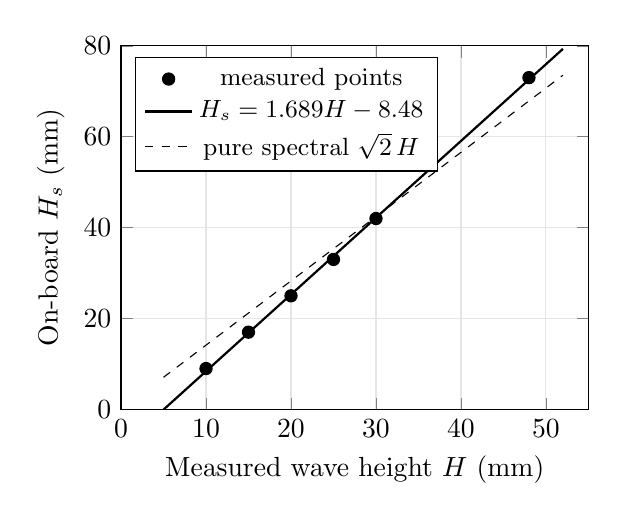
\begin{tikzpicture}
\begin{axis}[width=0.62\textwidth, height=6.2cm,
  xlabel={Measured wave height $H$ (mm)}, ylabel={On-board $H_s$ (mm)},
  xmin=0, xmax=55, ymin=0, ymax=80, grid=both, grid style={gray!20},
  legend pos=north west, legend style={font=\small}]
\addplot[only marks, mark=*, mark size=2.2pt] coordinates
  {(10,9) (15,17) (20,25) (25,33) (30,42) (48,73)};
\addlegendentry{measured points}
\addplot[thick, domain=5:52] {1.6886*x - 8.4845};
\addlegendentry{$H_s = 1.689H - 8.48$}
\addplot[dashed, domain=5:52] {1.414*x};
\addlegendentry{pure spectral $\sqrt{2}\,H$}
\end{axis}
\end{tikzpicture}
\caption{Height response at \SI{0.5}{\hertz}. The fitted slope (1.689) exceeds the
monochromatic spectral expectation ($H_s = \sqrt{2}H \approx 1.414H$) by a factor
1.19, attributed to platform response at this frequency; the negative intercept
represents a fixed $\sim$\SI{5}{\milli\meter} of surface motion (in $H$ units,
$-b/a$) not transduced by the buoy.}
\label{fig:height}
\end{figure}

\paragraph{Interpretation.} For a monochromatic wave of height $H$, the
spectral definition $H_s = 4\sqrt{m_0}$ yields $H_s = \sqrt{2}\,H$
\citep{holthuijsen2007,longuethiggins1952}. The fitted slope of 1.689 implies
the buoy transduced vertical motion $\approx 1.19\times$ the true surface
motion at \SI{0.5}{\hertz} --- a modest platform-response (RAO) excess
consistent with a light, small buoy below but approaching its heave-response
peak. The negative intercept corresponds to $\approx \SI{5}{\milli\meter}$ of
surface height that produces no measured response, plausibly a combination of
tether restraint, surface tension on the hull, and processing losses at the
smallest amplitudes; it implies degraded relative accuracy for waves below
$\sim$\SI{10}{\milli\meter}.

\subsection{Period response}
\label{sec:period}
Table~\ref{tab:period} lists all frequencies achieved. The on-board period was
exact at every point to within the \SI{0.1}{\second} reporting grain, and the
underlying spectral peak matched the drive frequency within 2\% throughout ---
including through a taut tether at \SI{1.5}{\hertz} and in the basin-mode
regime at \SI{0.2}{\hertz}.

\begin{table}[h]
\centering
\caption{Period validation (all at \SI{3}{\volt} except as noted). Peak
frequency is the median settled on-board spectral peak; $T_p$ the reported
period. The \SI{0.667}{\second} case is grain-limited (reported grid is
\SI{0.1}{\second}); its spectral peak (\SI{1.53}{\hertz}) is within 2\%.}
\label{tab:period}
\begin{tabular}{S[table-format=1.1] S[table-format=1.3] S[table-format=1.1] S[table-format=1.3] l}
\toprule
{Drive freq.\ (\si{\hertz})} & {$T$ true (\si{\second})} & {$T_p$ (\si{\second})} & {Peak (\si{\hertz})} & {Notes} \\
\midrule
0.2 & 5.0   & 4.9 & 0.202 & untethered; basin-mode regime \\
0.4 & 2.5   & 2.5 & 0.410 & \SI{5}{\volt}, lowered water \\
0.5 & 2.0   & 2.0 & 0.510 & \\
1.0 & 1.0   & 1.0 & 1.020 & \\
1.5 & 0.667 & 0.7 & 1.530 & tether taut (flagged) \\
\bottomrule
\end{tabular}
\end{table}

\subsection{Transfer validation at 0.4\,Hz}
\label{sec:transfer}
With the water level lowered and the paddle at its \SI{5}{\volt} maximum, a
$T = \SI{2.5}{\second}$ wave was generated and measured at the buoy at
$H = \SIrange{30}{35}{\milli\meter}$ (video-ruler band). The settled on-board
estimate was $H_s = \SI{50}{\milli\meter}$; applying the inverse of
Eq.~(\ref{eq:affine}) gives
\[
  \hat H = \frac{50 + 8.48}{1.689} = \SI{34.6}{\milli\meter},
\]
inside the measured band. The calibration fitted at \SI{0.5}{\hertz} therefore
transfers to \SI{0.4}{\hertz} at $\sim$1.5$\times$ the fitted amplitude
mid-range and in a different depth regime, within ground-truth uncertainty.

\subsection{Spectral observations}
\label{sec:seiche}

\paragraph{Basin seiche.} During early testing with a wide filter band, the
$H_s$ estimate was intermittently dominated by energy at \SI{0.097}{\hertz}.
Merian's formula for the fundamental longitudinal seiche of a closed
rectangular basin, $T = 2L/\sqrt{gd}$ \citep{rabinovich2009}, gives
\SI{0.099}{\hertz} for $L = \SI{10}{\meter}$, $d = \SI{0.4}{\meter}$ ---
identifying the contamination as the tank's fundamental seiche and,
incidentally, providing an independent estimate of the working depth. The
filter low edge was subsequently placed above the seiche
(\SIrange{0.15}{0.3}{\hertz} depending on test), which removed the
contamination. The second longitudinal mode is predicted near
\SI{0.2}{\hertz}; long-period forcing at \SIrange{0.2}{0.2}{\hertz}
consequently produced a partly standing basin response with strong spatial
amplitude variation, and long-period height measurements should be regarded
as position-specific.

\paragraph{Harmonic content at large stroke.} At \SI{3}{\volt} drive and
\SI{0.5}{\hertz}, off-line spectral decomposition of the raw
\SI{10}{\hertz} heave record showed 70.8\% of in-band acceleration energy at
the fundamental (\SI{0.51}{\hertz}), 20.1\% at the first harmonic
(\SI{1.0}{\hertz}), and 6.1\% above --- the signature of finite-amplitude
(Stokes-type) wave steepening rather than facility noise (cross-tank sloshing
at the predicted \SI{0.8}{\hertz} band contributed only 1.3\%). Because the
on-board height estimate converts acceleration to elevation at a single
reference frequency, harmonic energy is over-weighted at conversion
($\propto (f/f_p)^4$); a per-bin conversion is recommended
(\S\ref{sec:recs}).

\paragraph{Platform resonance indication.} At fixed \SI{3}{\volt} drive, the
sensed $H_s$ at \SI{1.0}{\hertz} (\SI{83}{\milli\meter}) was double the
\SI{0.5}{\hertz} value (\SI{42}{\milli\meter}). Without an independent height
measurement at \SI{1.0}{\hertz} the wavemaker transfer and platform response
cannot be separated, but combined with morning free-float observations (buoy
heave $\approx 1.4\times$ surface at $T = \SI{1}{\second}$), a buoy heave
resonance in the vicinity of \SI{1}{\hertz} is the working hypothesis. A
response-amplitude-operator (RAO) determination with independent wave-probe
ground truth versus frequency is the definitive follow-up
\citep{raghukumar2019}.

\subsection{Operating-envelope findings}
\label{sec:envelope}
\begin{itemize}
  \item \textbf{Facility ceiling.} Above $\sim$\SI{1.5}{\hertz} the basin
        response became irregular (short waves reflect strongly from an
        absorbing beach tuned for longer waves); \SI{2.0}{\hertz} forcing
        produced no stable spectral peak at the buoy and the points were
        abandoned. This is a facility limit, not an instrument limit.
  \item \textbf{Tether loading.} The slack cross-tank tether went taut at
        $\ge$\SI{1.5}{\hertz} (drift force grows steeply with frequency).
        The period estimate was unaffected; height data under taut tether are
        flagged damped/suspect.
  \item \textbf{Free-drift envelope.} Untethered, the buoy crossed the
        available half-tank in under \SI{3}{\minute} at \SI{2}{\hertz}
        (faster than one estimator window), but drifted slowly enough at
        $\le$\SI{0.5}{\hertz} for clean untethered points.
  \item \textbf{Detection floor.} The smallest wave tested
        ($H = \SI{10}{\milli\meter}$, peak acceleration
        $\sim$\SI{0.05}{\meter\per\second\squared}) was detected with strong
        spectral prominence (period lock throughout); the practical floor is
        set by the affine intercept rather than by detection.
  \item \textbf{Run hygiene.} Automated frequency-detection bracketing
        eliminated two classes of labeling error observed under manual
        timing (operator-missed steps; clock skew). An instrument-side
        window reset on run start was identified as unnecessary dead time
        and disabled server-side mid-campaign; transitions are instead
        excluded in scoring.
\end{itemize}

\section{Discussion}
The instrument's period channel is field-ready: five frequencies spanning
\SIrange{0.2}{1.5}{\hertz} (periods \SIrange{0.7}{5}{\second}) were reported
exactly at instrument resolution, through tether loading, harmonic
contamination, and basin-mode conditions. This is the primary quantity for
the sargassum-drift application.

The height channel is usable with the affine calibration of
Eq.~(\ref{eq:affine}), which held with sub-millimetre residuals over a
$5\times$ height range and transferred to an independent frequency/amplitude/
depth point. Two caveats bound its validity: (i)~the slope contains a
platform-response factor measured at \SIrange{0.4}{0.5}{\hertz}; near the
suspected $\sim$\SI{1}{\hertz} resonance the effective slope is larger
(under-estimating true height if the tank calibration is applied
unmodified), and at long ocean swell periods
($\ge$\SI{5}{\second}) the platform follows the surface nearly perfectly, so
the slope should relax toward the spectral $\sqrt{2}$; a per-frequency
correction table is the appropriate refinement. (ii)~the negative intercept
implies a $\sim$\SI{5}{\milli\meter} height floor below which relative error
grows rapidly --- immaterial for ocean swell but relevant to tank work.

All conclusions rest on monochromatic seas. The estimator's field task ---
extracting the energetic peak from a mixed swell-plus-wind-sea spectrum ---
was not exercised here and is the highest-value follow-up test (the facility
can superimpose wind chop on paddle swell).

\section{Conclusions}
\begin{enumerate}
  \item Peak-period reporting is validated across \SIrange{0.7}{5.0}{\second}
        with $\le 2\%$ spectral-peak error at every achievable facility
        frequency.
  \item On-board $H_s$ follows an affine law in true height at
        \SI{0.5}{\hertz}: $H_s = 1.689H - 8.48$~mm
        ($R^2 = 0.9995$); the inverse map recovers true height to
        $\sim$\SI{1}{\milli\meter} in-sample and validated at
        \SI{0.4}{\hertz} within ground-truth uncertainty.
  \item The flume's fundamental seiche (\SI{0.097}{\hertz} measured;
        \SI{0.099}{\hertz} Merian) was identified and excluded by filter-band
        placement; band edges must bracket the wave band with margin at both
        ends (two edge-collision incidents during the campaign).
  \item Facility limits: clean monochromatic operation
        \SIrange{0.2}{1.5}{\hertz}; irregular above; long-period forcing is
        basin-mode dominated and position-dependent.
  \item Platform heave response likely peaks near \SI{1}{\hertz}; an RAO
        determination and mixed-sea (wind) validation are the recommended
        next campaigns.
\end{enumerate}

\section{Recommendations}
\label{sec:recs}
\begin{enumerate}
  \item \textbf{Firmware: runtime calibration constants.} Expose the affine
        pair $(a, b)$ as persisted, remotely settable parameters applied at
        reporting time (raw $H_s$ retained in telemetry), replacing the
        current display-side application.
  \item \textbf{Firmware: per-bin spectral conversion.} Convert acceleration
        to elevation per FFT bin ($/\omega^4$ in power) before band
        integration, removing the harmonic over-weighting of
        \S\ref{sec:seiche}.
  \item \textbf{Firmware: remove run-start window reset} (already neutralized
        operationally) and add band-edge sanity warnings when the spectral
        peak approaches either filter edge.
  \item \textbf{Testing: RAO campaign} --- independent wave-probe ground
        truth versus frequency at fixed height, to convert the single-point
        platform-response factor into a response curve.
  \item \textbf{Testing: mixed-sea validation} --- paddle swell plus wind
        chop; verify the prominence-gated $T_p$ locks the energetic swell
        peak and characterize $H_s$ behaviour in bimodal spectra.
  \item \textbf{Ocean preset.} For deployment, shift the filter band to the
        ocean swell/wind-sea range ($\sim$\SIrange{0.05}{0.5}{\hertz});
        re-derive the platform-response slope for long-period swell (expected
        $\to \sqrt{2}$).
\end{enumerate}

\begin{thebibliography}{9}
\bibitem[Holthuijsen(2007)]{holthuijsen2007}
Holthuijsen, L.~H. (2007). \emph{Waves in Oceanic and Coastal Waters}.
Cambridge University Press.

\bibitem[Longuet-Higgins(1952)]{longuethiggins1952}
Longuet-Higgins, M.~S. (1952). On the statistical distribution of the heights
of sea waves. \emph{Journal of Marine Research}, 11(3), 245--266.

\bibitem[Rabinovich(2009)]{rabinovich2009}
Rabinovich, A.~B. (2009). Seiches and harbour oscillations. In Y.~C. Kim
(Ed.), \emph{Handbook of Coastal and Ocean Engineering} (pp.~193--236).
World Scientific.

\bibitem[Raghukumar et al.(2019)]{raghukumar2019}
Raghukumar, K., Chang, G., Spada, F., Jones, C., Janssen, T., \& Gans, A.
(2019). Performance characteristics of ``Spotter,'' a newly developed
real-time wave measurement buoy. \emph{Journal of Atmospheric and Oceanic
Technology}, 36(6), 1127--1141. \texttt{doi:10.1175/JTECH-D-18-0151.1}

\bibitem[WMO(2018)]{wmo702}
World Meteorological Organization (2018). \emph{Guide to Wave Analysis and
Forecasting} (3rd ed.), WMO-No.~702. Geneva.

\bibitem[Dean \& Dalrymple(1991)]{deandalrymple1991}
Dean, R.~G., \& Dalrymple, R.~A. (1991). \emph{Water Wave Mechanics for
Engineers and Scientists}. World Scientific.
\end{thebibliography}

\appendix
\section{Campaign notes and discarded data}
\label{sec:discarded}
An initial height sweep (six points, \SIrange{10}{48}{\milli\meter} nominal)
was conducted with live by-eye ruler readings as ground truth. Midway through
the campaign the field team determined that this method systematically
under-read wave height; the entire first sweep was voided and repeated with
the video-ruler protocol. Data from the voided sweep were internally
self-consistent (the on-board estimates tracked a straight line) but are
excluded from all fits. One period-sweep point was additionally re-measured
after an operator-side missed step was caught by the instrument itself (the
telemetry showed the spectral peak unchanged at the prior frequency),
motivating the switch to detection-based run bracketing used for the rest of
the campaign.

\section{Board configuration}
Sampling \SI{10}{\hertz}; window $N = 1024$ (\SI{102.4}{\second});
band-pass low edge 0.08 / 0.15 / 0.30~\si{\hertz} and high edge 0.5 / 2.0 /
3.0~\si{\hertz} across campaign phases (final long-period configuration
\SIrange{0.15}{3.0}{\hertz}); $T_p$ prominence gate 10.0 (default), median
filter $n = 5$; telemetry \SI{2}{\hertz}; timestamps server-side at receipt.
\end{document}
